% Exercise Template
% A LaTeX template for typesetting exercise in Persian (with cover page).
% By: Reza Adinepour
% Github: github.com/rezaAdinepour

\documentclass[12pt]{exam}

\usepackage{setspace}
\usepackage{listings}
\usepackage{graphicx,wrapfig}
\usepackage{caption}
\usepackage{subcaption}
\usepackage{multirow}
\usepackage{matlab-prettifier}
\usepackage{amsmath}
\usepackage{multicol}
\usepackage[hidelinks]{hyperref}



\usepackage[utf8]{inputenc}
\usepackage{fourier} 
\usepackage{array}
\usepackage{makecell}

\renewcommand\theadalign{bc}
\renewcommand\theadfont{\normalsize}
\renewcommand\theadgape{\Gape[4pt]}
\renewcommand\cellgape{\Gape[4pt]}


\usepackage[margin=25mm]{geometry}
\usepackage{xepersian}
\settextfont{XB Niloofar}

\newcommand{\class}{\ThesisClass}

\singlespacing
\parindent 0ex

\begin{document}


% -------------------------------------------------------
%  Thesis Information
% -------------------------------------------------------

\newcommand{\ThesisType}
{سمینار}  % پایان‌نامه / رساله
\newcommand{\ThesisDegree}
{کارشناسی ارشد گرایش معماری کامپیوتر}  % کارشناسی / کارشناسی ارشد / دکتری
\newcommand{\ThesisMajor}
{مهندسی کامپیوتر}  % مهندسی کامپیوتر
\newcommand{\ThesisTitle}
{تمرین شبیه‌سازی سری ۳}
\newcommand{\ThesisAuthor}
{\href{https://github.com/rezaAdinepour/M.Sc-AUT/tree/main/Advanced Computer Architecture}{\textcolor{black}{رضا آدینه پور}} - ۴۰۲۱۳۱۰۵۵}
\newcommand{\ThesisSupervisor}
{جناب آقای دکتر فربه}
\newcommand{\ThesisDate}
{۲۳ آذر ۱۴۰۲}
\newcommand{\ThesisDepartment}
{دانشکده مهندسی کامپیوتر}
%\newcommand{\ThesisUniversity}
%{دانشگاه صنعتی امیرکبیر}

% -------------------------------------------------------
%  English Information
% -------------------------------------------------------

%\newcommand{\EnglishThesisTitle}{A Standard Template for Course Exercise}


\pagestyle{empty}

\begin{center}


\includegraphics[scale=0.15]{images/aut-fa.png}

%\vspace{0.5cm}
%\ThesisUniversity \\[-0.3em]
%\vspace{0.5cm}
\large\ThesisDepartment

\begin{large}
\vspace{0.5cm}


%\ThesisMajor

\end{large}

\vspace{1.5cm}

{عنوان:}\\[1.2em]
{\LARGE\textbf{\ThesisTitle}}\\ 
\vspace{1cm}
% \begin{latin}
% {\Large\textbf\EnglishThesisTitle}
% \end{latin}

\vspace{2cm}

{نگارش}\\[.5em]
{\large\textbf{\ThesisAuthor}}

\vspace{1.5cm}

{استاد مربوطه}\\[.5em]
{\large\textbf{\ThesisSupervisor}}

\vspace{1cm}



\vspace{2cm}

\ThesisDate

\end{center}

\newpage


% These commands set up the running header on the top of the exam pages
\pagestyle{head}
\firstpageheader{}{}{}
\runningheader{صفحه \thepage\ از \numpages}{}{\class}
\runningheadrule

\vspace{0pt}


\begin{questions}
	\pointpoints{نمره}{نمره}
	
	\section*{سوالات تئوری}
	\question
\textbf{به سوالات زیر پاسخ دهید:‌ }

\begin{enumerate}
	\item 
	\lr{PUM} چیست و کدام نوع حافظه‌ها برای آن بیشتر استفاده می‌شوند؟ توضیح دهید چرا هر نوع حافظه استفاده می‌شود.
	
	\textbf{پاسخ: }
پردازش در حافظه (\lr{PUM}) یک کانسپت محاسباتی است که در آن برخی از محاسبات ساده مانند جمع و ضرب به جای انتقال داده‌ها بین \lr{CPU} و حافظه، مستقیما در حافظه انجام می‌شوند.

معمولا از \lr{DRAM}، \lr{SRAM} و \lr{NVM} ها در \lr{PUM} استفاده می‌شود. که در ادامه به بررسی مزایا و معایب استفاده از هرکدام می‌پردازیم.

\lr{DRAM} ها
به دلیل اینکه رایج‌ترین نوع حافظه فرار با تراکم بالا و هزینه کم به ازای هر بیت هستند، به طور گسترده استفاده می‌شود. ویژگی‌های خازنی سلول‌های \lr{DRAM} امکان انجام تکنیک‌های محاسباتی درون حافظه مانند عملیات منطقی و حسابی را فراهم می‌کند.

مزایا: تراکم بالا، ارزان است.\\
معایب: فرار، نیاز به تازه‌سازی دوره‌ای و معمولاً تأخیر بیشتر نسبت به \lr{SRAM}.

اما در مقابل  \lr{SRAM} زمان‌های تأخیر کمتری و زمان دسترسی سریعتری نسبت به \lr{DRAM} دارد و در مواردی که سرعت برای ما بسیار مهم است، (مانند \lr{Cache})، استفاده می‌شود. توانایی حفظ حالت بدون نیاز به تازه‌سازی، آن را برای عملیات‌های \lr{PUM} مناسب می‌سازد.

مزایا: زمان‌های دسترسی سریع نسبت به \lr{DRAM}، عدم نیاز به تازه‌سازی.\\
معایب: تراکم کمتر و هزینه بیشتر به ازای هر بیت نسبت به \lr{DRAM}.


درمقابل حافظه‌های فرار، انواع حافظه‌های غیر فرار مانند \lr{Flash}، \lr{PCM} و \lr{ReRAM} به دلیل نگه داشتن داده بدون برق، برای ذخیره‌سازی پایدار و محاسبات مناسب هستند. این حافظه‌ها می‌توانند برخی عملیات منطقی را درون سلول‌های حافظه انجام دهند.

مزایا: غیر فرار بودن. \\
معایب: عموماً سرعت نوشتن کندتر و دوام کمتر نسبت به \lr{DRAM} و \lr{SRAM}.
	
	
	
	
	
	\item 
	نقاط ضعف \lr{UPMEM} چیست؟
	
	\textbf{پاسخ:} از نقاط ضعف \lr{UPMEM} ها می‌توان به موارد زیر اشاره کرد:
	
	
	\begin{enumerate}
		\item انعطاف‌پذیری و قابلیت برنامه‌ریزی محدود:\\
معماری \lr{PIM UPMEM} برای انواع خاصی از عملیات (مانند وظایف داده‌محور مانند جست‌وجو در پایگاه داده و تحلیل) است. ممکن است به اندازه CPU یا GPUهای سنتی عمومی و همه‌منظوره نباشد، که کاربرد آن را به بارهای کاری خاص محدود می‌کند.
		
		
		
		\item یکپارچه‌سازی و سازگاری:\\
یکپارچه‌سازی ماژول‌های \lr{PIM UPMEM} با سیستم‌های موجود می‌تواند چالش‌برانگیز باشد. ممکن است مشکلات سازگاری با معماری‌های حافظه و پردازنده فعلی به وجود بیاید که نیاز به اصلاحات در کانفیگ نرم‌افزار و سخت‌افزار دارد.
		
		
		
		\item مسائل مربوط به کارایی انرژی:\\
در حالی که \lr{PIM} هدفش کاهش مصرف انرژی با حداقل‌کردن حرکت داده‌ها بین حافظه و \lr{CPU} است،‌ صرفه‌جویی واقعی در انرژی می‌تواند وابسته به بار کاری باشد. برخی عملیات ممکن است همچنان مصرف انرژی قابل توجهی داشته باشند، به خصوص اگر منطق \lr{PIM} به‌طور کامل برای آن کاربرد به‌خصوص بهینه‌سازی نشده باشد.
		
		
		
		\item توسعه و اشکال‌زدایی:\\
همانطور که در کلاس هم بررسی شد، توسعه برنامه‌ها برای \lr{PIM} نیاز به مدل‌های برنامه‌نویسی و ابزارهای جدید دارد. دیباگ و پروفایل‌کردن برنامه‌های \lr{PIM} می‌تواند به دلیل طبیعت توزیع‌شده و درون حافظه‌ای محاسبات سخت‌تر از برنامه‌نویسی \lr{CPU/GPU} سنتی باشد.
		
	\end{enumerate}
	
	
	\item 
	ساختار \lr{Ambit} را معرفی کرده و مزایا و معایب آن را توضیح دهید.
	
	\textbf{پاسخ:} 
	\lr{Ambit}
یک معماری \lr{PIM} است که از بستر \lr{DRAM} موجود برای انجام عملیات بیتی (مانند \lr{AND}, \lr{OR}, \lr{NOT}) به طور مستقیم درون حافظه استفاده می‌کند. این معماری از ویژگی‌های آنالوگ سلول‌های \lr{DRAM} و \lr{Sense Amplifier} برای اجرای این عملیات استفاده می‌کند.

از مزایای آن می‌توان به موارد زیر اشاره کرد:

\begin{enumerate}
	\item کاهش حرکت داده‌ها:\\
با انجام محاسبات مستقیما درون \lr{DRAM} به طور قابل توجهی نیاز به حرکت داده بین \lr{CPU} و حافظه را کاهش می‌دهد، که منجر به کاهش تاخیر و مصرف انرژی می‌شود.

	\item توان محاسباتی بالا:\\
	\lr{Ambit}
می‌تواند عملیات بیتی را بر روی حجم زیادی از داده‌ها به طور همزمان انجام دهد، که توان محاسباتی بالایی برای وظایف داده‌محور مانند جستجوهای پایگاه داده، رمزنگاری و شبکه‌های عصبی فراهم می‌کند.


	\item تغییرات سخت‌افزاری حداقلی:\\
	\lr{Ambit}
از زیرساخت \lr{DRAM} موجود با تغییرات حداقلی استفاده می‌کند، که ادغام آن را با سیستم‌های فعلی نسبت به معماری‌های \lr{PIM} آسان‌تر می‌کند.
\end{enumerate}


همچنین از معایب \lr{Ambit} می‌توان به موارد زیر اشاره کرد:

\begin{enumerate}
	\item محدودیت در انواع عملیات:\\
	\lr{Ambit}
به طور عمده برای عملیات بیتی طراحی شده است. نمی‌تواند به طور کارآمد محاسبات پیچیده‌تر ریاضی یا اعشاری را انجام دهد، که کاربرد آن را به انواع خاصی از عملیات ها محدود می‌کند.


	\item پیچیدگی در برنامه‌نویسی:\\
برنامه‌نویسی برای \lr{Ambit} نیاز به درک مدل عملیاتی خاص و محدودیت‌های آن دارد. برنامه‌نویس ها باید الگوریتم‌های خود را برای استفاده موثر از عملیات بیتی تطبیق دهند، که می‌تواند پیچیدگی نرم‌افزاری را افزایش دهد.

	\item چالش‌های مقیاس‌پذیری:\\
در حالی که \lr{Ambit} توان محاسباتی بالایی برای عملیات بیتی ارائه می‌دهد، مقیاس‌پذیری آن به سیستم‌های حافظه بزرگ‌تر یا ادغام آن با واحدهای پردازشی دیگر ممکن است چالش‌هایی از نظر هماهنگی و مدیریت ایجاد کند.
\end{enumerate}


\end{enumerate}

%\begin{figure}[h]
%	\centering
%	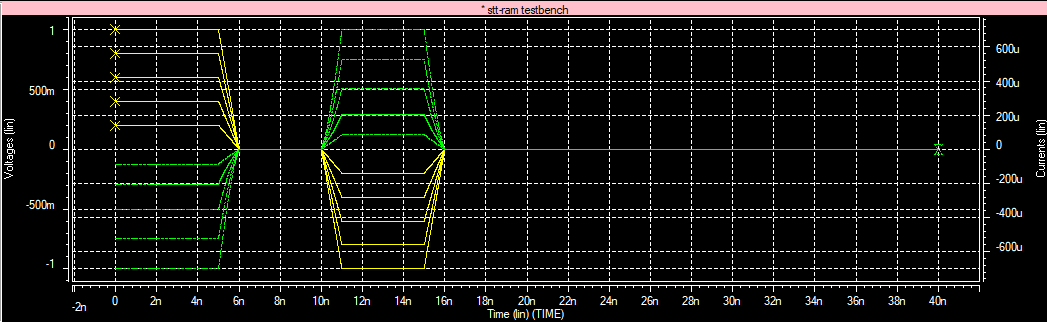
\includegraphics[width=1\textwidth]{images/img8}
%	\caption{خروجی شبیه‌سازی}
%	\label{خروجی شبیه‌سازی}
%\end{figure}

		
		
		
		
		
		
	\section*{سوالات شبیه‌سازی}
	\question
	
	
در این بخش از تکلیف خود، شما با شبیه‌ساز \lr{MNSIM 2.0} برای پیاده‌سازی یک شتاب‌دهنده شبکه عصبی سر و کار خواهید داشت. بنابراین، ابتدا باید این شبیه‌ساز را دانلود کرده و نتایج را طبق درخواست ارائه دهید.
	
	\subsection*{پیکربندی پایه:}
	\begin{enumerate}
		\item پارامتر‌های شبکه‌عصبی \lr{VGG8} که بر روی مجموعه داده \lr{CIFAR-10} آموزش دیده است را دانلود کنید، همانطور که در راهنمای \lr{MNSIM 2.0} توضیح داده شده است.
		\item برای هر اجرا، باید \lr{VGG8} را به عنوان شبکه عصبی مورد نظر خود انتخاب کنید.
	\end{enumerate}
	
	\textbf{پاسخ:} وزن ها را از \href{https://onedrive.live.com/?authkey=%21ANiQIk04073Gdfo&id=8F6F3FD340AC68D1%21332&cid=8F6F3FD340AC68D1}{\textcolor{magenta}{اینجا}}
	دانلود می‌کنیم.
	
	\subsection*{سوال 1:}
	
	همانطور که در کلاس یاد گرفتید، ساختار PIM شامل تعدادی کاشی است و هر کاشی شامل تعدادی PE است. در هر PE، ما مدارهای ضروری و ساختار ضربدری سلول‌های حافظه را داریم. اگر اندازه ضربدری را کاهش دهیم چه اتفاقی می‌افتد؟ به عنوان مثال، آیا باید انتظار داشته باشیم که توان، تأخیر و دقت کاهش، افزایش یا تغییر نکند؟ پاسخ خود را به تفصیل توضیح دهید.
	
	\subsection*{سوال 2:}
	
	اگر بخواهیم PUM را به این شبیه‌ساز اضافه کنیم، کدام قسمت باید تغییر کند؟
	
	\subsection*{سوال 3:}
	
	در اولین پیاده‌سازی، ابعاد ضربدری (Xbar) را به 256x256 تنظیم کنید. در پیاده‌سازی دوم، ابعاد ضربدری را به 128x128 تغییر دهید. مجموع تأخیر، توان و انرژی را گزارش دهید و جدول را پر کنید. چه اتفاقی افتاد؟ چرا؟ (برای هر پارامتر به تفصیل توضیح دهید.)
	
	\begin{table}[h]
		\centering
		\begin{tabular}{|c|c|c|c|}
			\hline
			& \textbf{128*128} & \textbf{256*256} & \textbf{وضعیت} \\ \hline
			\textbf{تأخیر} & & & کاهش / افزایش \\ \hline
			\textbf{توان} & & & کاهش / افزایش \\ \hline
			\textbf{انرژی} & & & کاهش / افزایش \\ \hline
		\end{tabular}
		\caption{جدول I}
	\end{table}
		
	
 \end{questions}

\end{document}